%\begin{figure}[htb]
%    \begin{center}
%        \begin{circuitikz}
%            \begin{scope}[yshift=-9cm, local bounding box=sawtooth]
                %\draw (0,-1) -- ++(0,2) -- ++(2,-2) -- ++(0,2) -- ++(2,-2) -- ++(0,2) -- ++(2,-2);
                % the above line does the same as the following one, but without the foreach loop
%                \draw (0,-1) foreach \x in {1,2,3} {-- ++(2,2) -- ++(0,-2) };
%            \end{scope}
%        \end{circuitikz}
%    \end{center}
%    \caption{Single-phase DC Inverter}
   % \label{fig:Fig_Single-phase_DC_Inverter}
%\end{figure}
%%%%%%%%%%%%%%%%%%%%%%%%%%%%%%%%%%%%%%%%%%%%%%%%%%%%%%%%%%%%%%%%%%%%%%%%%%
% Fundamental Current i^1_1a for M3C with RL-Load
%%%%%%%%%%%%%%%%%%%%%%%%%%%%%%%%%%%%%%%%%%%%%%%%%%%%%%%%%%%%%%%%%%%%%%%%%%
\begin{figure}[h]

    %   \documentclass{standalone}
    %   \usepackage{pgfplots}
    %   \pgfplotsset{compat=1.18} % Kompatibilität für neuere Versionen
           \centering
           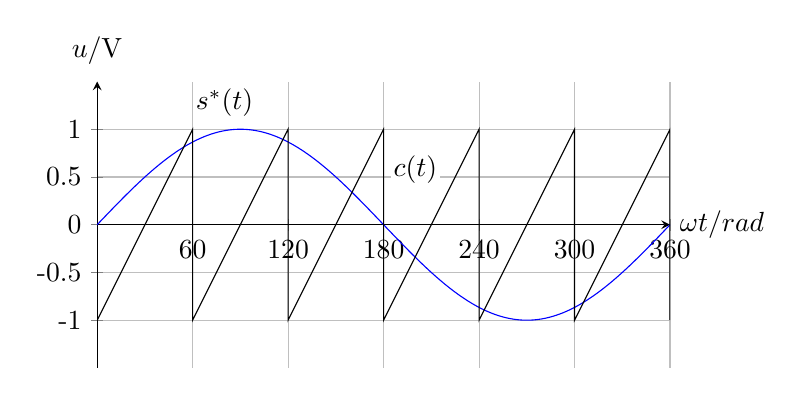
\begin{tikzpicture}
                \pgfplotsset{set layers}
           \begin{axis}[
            % x/y range adjustment
            scale only axis,
            ymin=-1.5, ymax=1.5,
            xmin=0, xmax=360, 
            samples=500,
            axis y line=center,
            axis x line=middle,
            extra y ticks=0,
            % Label text
            xlabel={$\omega t / \text{rad}$},
            ylabel={$u/\mathrm{V}$},
            % Label adjustment
            x label style={at={(axis description cs:1,0.5)},anchor=west},
            y label style={at={(axis description cs:0,.97)},anchor=south,yshift=0.2cm},
            width=0.6\textwidth,
            height=0.3\textwidth,
            % x-Ticks
            xtick={0,60,120,180,240, 300, 360},
            xticklabels={0,60,120,180,240, 300, 360},
            xticklabel style = {anchor=north},
            % y-Ticks
            ytick={-1,-0.5,0,0.5,1},
            yticklabels={-1,-0.5,0,0.5,1},
            yticklabel style = {anchor=east},
            % Grid layout
            grid,
            %grid style={line width=.1pt, draw=gray!10},
            %major grid style={line width=.2pt,draw=gray!90},
        ] 
        % modulation s
        \addplot[blue, domain= 0:360, solid] {sin(x)};
      % carrier signal c
       \draw[thin, black] (0,-1) -- (60,1) -- (60,-1) -- (120,1) -- (120,-1) -- (180,1) -- (180,-1) -- (240,1) -- (240,-1) -- (300,1) -- (300,-1) -- (360,1) -- (360,-1);
        %\draw (0,-1) \foreach \x in {0 ,60, 120, 180, 240, 300} {-- ++(60,2) -- ++(0,-2) };
        
        % Label of s
        \node[black, fill=white, inner sep = 1pt, anchor = south] at (axis cs:80,1.1) {$s^{*}(t)$};
        % Label of c
        \node[black, fill=white, inner sep = 1pt, anchor = south] at (axis cs:200,0.4) {$c(t)$};
           \end{axis}         
           \end{tikzpicture}
           \caption{Carrier signal $c(t)$ and reference $s^{*}(t)$.}
           \label{sfig:ex07_sub1.1_modulation}
   \end{figure}